\begin{figure}[H]
    \centering
    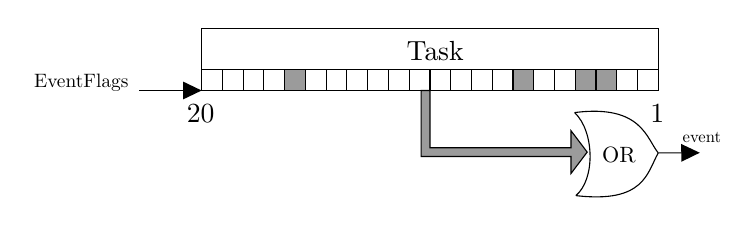
\begin{tikzpicture}[x=0.75pt,y=0.75pt,yscale=-1,xscale=1]
        \draw   (100,120) -- (110,120) -- (110,130) -- (100,130) -- cycle ;
        \draw   (110,120) -- (120,120) -- (120,130) -- (110,130) -- cycle ;
        \draw   (120,120) -- (130,120) -- (130,130) -- (120,130) -- cycle ;
        \draw   (130,120) -- (140,120) -- (140,130) -- (130,130) -- cycle ;
        \draw  [fill={rgb, 255:red, 155; green, 155; blue, 155 }  ,fill opacity=1 ] (140,120) -- (150,120) -- (150,130) -- (140,130) -- cycle ;
        \draw   (150,120) -- (160,120) -- (160,130) -- (150,130) -- cycle ;
        \draw   (160,120) -- (170,120) -- (170,130) -- (160,130) -- cycle ;
        \draw   (170,120) -- (180,120) -- (180,130) -- (170,130) -- cycle ;
        \draw   (180,120) -- (190,120) -- (190,130) -- (180,130) -- cycle ;
        \draw   (190,120) -- (200,120) -- (200,130) -- (190,130) -- cycle ;
        \draw   (200,120) -- (210,120) -- (210,130) -- (200,130) -- cycle ;
        \draw   (210,120) -- (220,120) -- (220,130) -- (210,130) -- cycle ;
        \draw   (220,120) -- (230,120) -- (230,130) -- (220,130) -- cycle ;
        \draw   (230,120) -- (240,120) -- (240,130) -- (230,130) -- cycle ;
        \draw   (240,120) -- (250,120) -- (250,130) -- (240,130) -- cycle ;
        \draw  [fill={rgb, 255:red, 155; green, 155; blue, 155 }  ,fill opacity=1 ] (250,120) -- (260,120) -- (260,130) -- (250,130) -- cycle ;
        \draw   (260,120) -- (270,120) -- (270,130) -- (260,130) -- cycle ;
        \draw   (270,120) -- (280,120) -- (280,130) -- (270,130) -- cycle ;
        \draw  [fill={rgb, 255:red, 155; green, 155; blue, 155 }  ,fill opacity=1 ] (280,120) -- (290,120) -- (290,130) -- (280,130) -- cycle ;
        \draw  [fill={rgb, 255:red, 155; green, 155; blue, 155 }  ,fill opacity=1 ] (290,120) -- (300,120) -- (300,130) -- (290,130) -- cycle ;
        \draw   (300,120) -- (310,120) -- (310,130) -- (300,130) -- cycle ;
        \draw   (310,120) -- (320,120) -- (320,130) -- (310,130) -- cycle ;
        \draw   (100,100) -- (320,100) -- (320,120) -- (100,120) -- cycle ;
        \draw    (70,130) -- (79.5,130) -- (98,130) ;
        \draw [shift={(100,130)}, rotate = 180] [fill={rgb, 255:red, 0; green, 0; blue, 0 }  ][line width=0.75]  [draw opacity=0] (8.93,-4.29) -- (0,0) -- (8.93,4.29) -- cycle    ;
        \draw    (320,160.06) .. controls (314.64,169.47) and (313.5,184.5) .. (280.29,180.64) ;
        \draw    (320,160.06) .. controls (314.4,153.47) and (312.16,136.5) .. (279.71,140.64) ;
        \draw    (280.29,180.64) .. controls (289.68,172.83) and (289.35,149.84) .. (279.71,140.64) ;
        \draw  [fill={rgb, 255:red, 155; green, 155; blue, 155 }  ,fill opacity=1 ] (210,130) -- (210,157.56) -- (277.94,157.56) -- (277.94,149.36) -- (285.75,159.68) -- (277.94,170) -- (277.94,161.8) -- (205.75,161.8) -- (205.75,130) -- cycle ;
        \draw    (320,160.06) -- (329.5,160.06) -- (338,160.01) ;
        \draw [shift={(340,160)}, rotate = 539.6700000000001] [fill={rgb, 255:red, 0; green, 0; blue, 0 }  ][line width=0.75]  [draw opacity=0] (8.93,-4.29) -- (0,0) -- (8.93,4.29) -- cycle    ;
        \draw (99.5,141) node  [align=left] {20};
        \draw (319.5,141) node  [align=left] {1};
        \draw (212.5,111) node  [align=left] {Task};
        \draw (42,126) node [scale=0.7] [align=left] {EventFlags};
        \draw (301,161) node [scale=0.8] [align=left] {OR};
        \draw (341,152.5) node [scale=0.6] [align=left] {event};
    \end{tikzpicture}
    \caption{Task event flags}
    \label{fig:eventflags}
\end{figure}